
%\newtheorem{definition}[subsection]{Definition}
%\newtheorem{example}[subsection]{Example}
\newtheorem{cor}[subsection]{Corollary}
\newtheorem{pro}[subsection]{Proposition}
\newtheorem{theo}[subsection]{Theorem}
\newtheorem{lem}[subsection]{Lemma}
%\newtheorem{rem}[subsection]{Remark}

\definecolor{main}{HTML}{5989cf}    % setting main color to be used
\definecolor{sub}{HTML}{cde4ff}     % setting sub color to be used

\tcbset{
    sharp corners,
    colback = white,
    before skip = 0.2cm,    % add extra space before the box
    after skip = 0.5cm      % add extra space after the box
}                           % setting global options for tcolorbox

% You can copy any following box you like to your code.
\newtcolorbox{boxA}{
    fontupper = \bf,
    boxrule = 1.5pt,
    colframe = black % frame color
}

\newtcolorbox{boxB}{
    fontupper = \bf\color{main}, % font color
    boxrule = 1.5pt,
    colframe = main,
    rounded corners,
    arc = 5pt   % corners roundness
}
\newtcolorbox{boxC}{
    colback = sub, % background color
    boxrule = 0pt  % no borders
}

\newtcolorbox{boxD}{
    colback = sub, 
    colframe = main, 
    boxrule = 0pt, 
    toprule = 3pt, % top rule weight
    bottomrule = 3pt % bottom rule weight
}

\hypersetup{
    colorlinks=true,
    linkcolor=blue,
    filecolor=magenta,      
    urlcolor=cyan,
    pdftitle={Overleaf Example},
    pdfpagemode=FullScreen,
    }

\urlstyle{same}


\coursetitle{\mtthreeiii}{MT303}
\developers{Wyclife Rao}
\reviewers{Dr. Irene Sitawa}
\modulenumber{5}
\modulename{Numerical Integration}

% courses
\thispagestyle{empty}
\begin{tikzpicture}[overlay,remember picture,font=\sffamily\bfseries]
 \draw[ultra thick,c4,name path=big arc] ([xshift=-2mm]current page.north) arc(150:285:11) coordinate[pos=0.225] (x0);
 \begin{scope}
  \clip ([xshift=-2mm]current page.north) arc(150:285:11) --(current page.north east);
  \fill[c4!50,opacity=0.25] ([xshift=4.55cm]x0) circle (4.55);
  \fill[c4!50,opacity=0.25] ([xshift=3.4cm]x0) circle (3.4);
  \fill[c4!50,opacity=0.25] ([xshift=2.25cm]x0) circle (2.25);
  \draw[ultra thick,c4!50] (x0) arc(-90:30:6.5);
  \draw[ultra thick,c4] (x0) arc(90:-30:8.75);
  \draw[ultra thick,c4!50,name path=arc1] (x0) arc(90:-90:4.675);
  \draw[ultra thick,c4!50] (x0) arc(90:-90:2.875);
  \path[name intersections={of=big arc and arc1,by=x1}];
  \draw[ultra thick,c4,name path=arc2] (x1) arc(135:-20:4.75);
  \draw[ultra thick,c4!50] (x1) arc(135:-20:8.75);
  \path[name intersections={of=big arc and arc2,by={aux,x2}}];
  \draw[ultra thick,c4!50] (x2) arc(180:50:2.25);
 \end{scope} 
 \path[decoration={text along path,text color=c4,
                 raise = -2.8ex,
                 text  along path,
                 text = {},%|\sffamily\bfseries|02/18/2019
                 text align = center,
             },
             decorate
         ] ([xshift=-2mm]current page.north) arc(150:245:11);
 %
 \newcommand\add{4cm}
 \begin{scope}%[shift={(5,0)}]
  \path[clip,postaction={fill=c3}]
  ([xshift=2cm+\add,yshift=-8cm]current page.center) rectangle ++ (4.6,7.7);
  \draw[c5,ultra thick,fill=c2] ([xshift=0.5cm+\add,yshift=-8cm]current page.center)
   ([xshift=0.5cm+\add,yshift=-8cm]current page.center)  arc(180:60:2)
    |- ++ (-3,6) --cycle;
  \draw[ultra thick,c5] ([xshift=-1.5cm+\add,yshift=-8cm]current page.center) 
  arc(180:0:2);
  \draw[ultra thick,c5] ([xshift=0.5cm+\add,yshift=-8cm]current page.center) 
  arc(180:0:2);
  \draw[ultra thick,c5] ([xshift=2.5cm+\add,yshift=-8cm]current page.center) 
  arc(180:0:2);
  \draw[ultra thick,c5] ([xshift=4.5cm+\add,yshift=-8cm]current page.center) 
  arc(180:0:2);
  \fill[white] ([xshift=2.5cm+\add,yshift=-8cm]current page.center) +(60:2) circle(1.5mm)
  node[above
  right=0mm,text=c5!80!black]{$\rho:=\dfrac{1+\sqrt{-3}}{2}$};
 \end{scope}
 %
 \fill[c1] ([xshift=2cm+\add,yshift=-8cm]current page.center) rectangle ++ (-30.7,7.7);
 \node[text=white,anchor=west,scale=2.3,inner sep=0pt] at
 ([xshift=-10cm,yshift=-1.8cm]current page.center) {\color{ulabgold} LEARNING};
 \node[text=white,anchor=west,scale=5,inner sep=0pt] at
 ([xshift=-10cm,yshift=-3.25cm]current page.center) {MODULE \dpmdnumber};
 \node[text=white,anchor=west,scale=2.5,inner sep=0pt,text width=.4\textwidth] at
 ([xshift=-10cm,yshift=-6cm]current page.center) {\dpmdname};
 \node[text=white,anchor=east,scale=2,inner sep=0pt] at
 ([xshift=5.7cm,yshift=-7.5cm]current page.center) {\color{ulabgold}The Open University of Kenya};
 %
% \draw[gray,line width=5mm] 
% ([xshift=2mm,yshift=-1mm]current page.south west) rectangle ([xshift=-2mm,yshift=1mm]current
% page.north east);
\end{tikzpicture}

%\newpage
\pagenumbering{roman}
\thispagestyle{empty}%firstpage


\begin{center}
\vspace*{2cm}
{\Huge\bf BACHELOR OF TECHNOLOGY EDUCATION}\\[3cm]  


%{\fontsize{80}{40}\selectfont \dpcoursecode}\\[2cm]
%
%{\fontsize{30}{40} \selectfont \dpcoursename}\\[2cm]

%\rule{\textwidth}{1pt}
%\vspace{2cm}

%{\fontsize{40}{40}\selectfont \bf Module~\dpmdnumber}\\[2cm]
%
%{\fontsize{30}{40}\selectfont \bf \dpmdname}\\

\vfill
\begin{flushright}
\begin{minipage}{.6\textwidth}
\begin{tcolorbox}%[text ]
\begin{tabular}{ll}%\hline
\subtitle{Developed by:}&\displaydevelopers\\
&\\
\subtitle{Reviewed by:}&\makecell[l]{\displayreviewers}\\
\end{tabular}
\end{tcolorbox}
\end{minipage}\hspace*{-3.5cm}
\end{flushright}
\vspace*{-2.5cm}
\end{center}

\newpage
\thispagestyle{empty}
\null
\vfill
{\renewcommand\arraystretch{1.5}
\begin{tabular}{|l|l|}\hline
\subtitle{Programme Title} & Bachelor of Technology Education \\\hline
\subtitle{Course Title} & \fullcoursename\\\hline
\subtitle{Learning Module number} & Module \dpmdnumber\\\hline
\subtitle{Learning module title} & \dpmdname \\\hline
\subtitle{Module Developer} & \displaydevelopers\\\hline
\subtitle{Reviewed by} & \displayreviewers\\\hline
%\subtitle{Vision} & \vision\\\hline
%\subtitle{Audience description} & \\\hline
\end{tabular}}
\clearpage

%\section{COURSE LEARNING GUIDE}


\subsection*{Preparing for Online and Distance Learning}

This course offers you the opportunity to enter an online space where you can engage with fellow students at the university. The online forums, exercises, tasks and materials have been designed by the course facilitators in such a way that you can draw directly from their knowledge and share in their scholarly interest in online learning and assessment

We hope you will use your access to this virtual classroom to raise all your questions on the course module, to build a network great learners and to share your own thoughts and experiences to the benefit of your fellow students.

   
There are a number of steps you can take to ensure you are well prepared to make the most of this learning opportunity. This resource should prompt you to consider the following:


 \begin{enumerate}[label=\cb$\square$]
   \item How can you best prepare the space where you expect you will spend most of your time engaging in online learning (i.e. in your home or office, or even during your commute to work or whilst traveling)?
  \item   What can you do to ensure you keep working through the course material, even when you do not have Internet access?
    \item How can you familiarise yourself with the course layout, in order to be able to navigate through the steps with ease?
    \item What are the communication strategies and best practices you could consider to best engage with your fellow students and the course facilitators?
    \item What do you do when you need academic or technical support?

 \end{enumerate} 

\subsection*{General Module Guide}

The authors of this module believe that imparting knowledge should always be a mutual relationship between the students and the teachers. Students can actively construct knowledge through experiences gained in reading and answering the learning modules.

You should take time to read everything written in the module, actively and religiously solve all the exercises included to finish this course and be able to gain all the competencies and skills expected to demonstrate the learning outcomes as stated in this course. If you finish with full confidence that you understand and can apply all the knowledge you gain in this course, then you are sure to succeed in tackling the next higher subjects in your chosen course.

In this course, you will be taught not only the knowledge you need to demonstrate your learning outcomes, but you will also gain discipline, perseverance, higher thinking skills, and resourcefulness that would help strengthen your foundation to succeed in life. To successfully finish the course, you must follow the guides set forth in using this module.


\begin{description}[{format=\textcolor{ulabblue}}]
\item[STUDY ENVIRONMENT.]\leavevmode\\
Before engaging into the module, make sure that you are comfortable enough and diminish distractions. Make sure that you develop a study routine to perform and accomplish all the activities set forth by the module.
%\newpage

\item[MODE OF DELIVERY.]\leavevmode\\
Students are required to get a access a digitised copy of the module from the Virtue Learning Environment. As an open and distance learner, you should be able to learn independently and optimise the learning modes and environment available to you as much of  the delivery of all the lessons will be done asynchronously. Your success will greatly depend on your self-motivation and discipline to get your work done without your instructor to remind you from time to time.

\item[STUDY SCHEDULE.] \leavevmode\\
Remember that you have other subjects to attend to, hence, you must manage your time so that you will not be left behind in any of them. Create your own learning plan for each course to make sure that you can perform all the activities. Do not procrastinate your work, remember that time wasted can never be retrieved back. Make sure that even if you are at home, you are a student enrolled in a program, where the learning of all its courses greatly depends on your will to learn as the materials you need are all in your hands. So always be aware of your daily tasks.

\item[PRACTICE EXERCISE.]\leavevmode\\
To measure your learning from your reading, you are given practice exercises which you are supposed to answer daily. This will prepare you in performing your main task.

\item[ONLINE GROUP CHAT.]\leavevmode\\
I am going to create an online Discussion Forum and QA Forum  on the VLE.  This will serve as a room for discussion on the topics and activities found in your module.

\item[RECOMMENDED REFERENCES FOR SUPPLEMENTARY READING.]\leavevmode\\
You are given links that you need to access online. These links are online references such as e-books, online activities, and tutorial videos of the topic. These are other references you can use to further understand the topic and gain additional knowledge and skills.

\item[MAIN TASK.]\leavevmode\\
You are given a task that will require you to apply the knowledge and skills you learned from the module. This can be a group or individual activity which will measure your higher order thinking skills you acquired throughout the topic.

\item[RUBRICS. ]\leavevmode\\
This is a tool to guide you in performing your main task. Through this, you will be able to know the specific indicators that should be found in your task. This is to assess your constructive behaviour towards your learning application. You will be rated according to a 4-point scale shown below.
\begin{center}
{\color{ulabgold} \bf 4 − Excellent\quad\quad   3 −Good\quad\quad    2 − Fair \quad\quad  1 −Poor}
\end{center}
\item[REFLECTIONS.]\leavevmode\\
Writing your reflection will be a passageway to express your experiential learning in using this module. In your honest recall, write everything that you think happened to you during your learning experience in this module. Use the guide questions below:
\begin{description}[{format=\textcolor{ulabblue}}]
\item[First paragraph. ]\leavevmode\\
How was your learning experience? Maybe you can consider describing the effect of the parts of the module (sequence, discussions, examples, practice exercises, online activities, and the main task) in your learning experience. You can point out the strength and weakness of each part so that we can consider it for future improvement of this instructional material.
\item[Second paragraph.  ]\leavevmode\\
What did you learn? Did you successfully acquire the learning outcomes?

\item[Third paragraph.]\leavevmode\\
How can you use what you learned in the future?
\end{description}
\end{description}

\section{ASSESSMENT  TASKS \& EXAMINATION   RULES AND GUIDELINES}

\begin{enumerate}[label=\cb\arabic*.]
\item {\cb SUBMISSION OF ASSESSMENT TASTS.}

Since mathematical skills are best acquired through constant practice, you are encouraged to answer at least two (2) exercises a day. These practice exercises will not be graded but it will help you develop your thinking skills which will prepare you in the performance of your main tasks. You are required to submit your practice exercises every week.
\begin{center} {\cg Usually submission deadlines are set on Saturday 11:59PM EAT} \end{center}

\item  {\cb GROUP CHAT.}

You can post questions, solutions, and comment to other's post. Please be reminded that our group chat is exclusive only for discussion on topics related to this course. Everyone is required to actively participate in the discussions. Also, trolling is highly discouraged. Always observe proper online etiquettes when participating in discussions.
\begin{center} {\cb RULE OF THUMB: ALWAYS THINK BEFORE YOU CLICK} \end{center}

\item  {\cb MAIN TASK. }

Complete documentation during the preparation of your task is required to ensure that every member of the group participated and contributed in the task. May it be photos or screenshots of your virtual meetings or group works. You are going to submit it as attachment of your main task the same way as the practice exercises.



\item {\cb RECOMMENDED REFERENCES FOR SUPPLEMENTARY READING.} 

You can explore online for other references that is related to the topic to gain additional information about the topic. Do not share or post inappropriate materials online or even privately.
\end{enumerate}

\subsection*{Requirements to pass the course}

Compiled Continuous  Assignment/Activities and Tasks  with Final Performance Examination.

\subtitle{Grading System}
\begin{center}
{\renewcommand\arraystretch{1.5}
\begin{tabular}{|l|c|}\hline
Continuous Activities and Tasks  &  50\%\\\hline
Final Performance Examination. &  50\%\\\hline
\end{tabular}
}
\end{center}
%\newpage










%\subsection{INTRODUCTORY MESSAGE}

%A warm welcome to \;  \fullcoursename, {\bf Module on \dpmdname}.



%By this module learning resource, we aim to enable you  achieve the relevant competencies, depict skill, action and purpose successfully. 
 

%It has been designed to provide you with fun and meaningful opportunities for guided and independent learning at your own pace and time. You will be enabled to process the contents of the learning material while being an active learner. Your academic success lies in your own hands.  This module has the following parts and corresponding icons:





{
\renewcommand\arraystretch{4}
\begin{longtblr}{
width=\linewidth,
 colspec={ Q[1,c,f] Q[1.5,r,m] Q[4,l,m] },
%row{1} = { font=\bfseries },
% rowhead = 1,
  caption={ }, 
  label={ },
  rowsep = 4pt,
  hlines = {ulabblue!20, 1pt},
  vlines = {ulabblue!20, 1pt},
}

\includegraphics[width=2cm]{img/audience} & {\bf AUDIENCE}  &  This is a description of a target audience.   \\
{\fontsize{40}{30}\selectfont\color{ulabblue}\faCogs}& {\bf MODULE DESCRIPTION} & 
This part explains the importance of the topics discussed in the module. It will also give you a sneak peek of what you will learn and what is expected from you at the end of the module.\\

\includegraphics[width=2cm]{img/target.png} &  {\bf  EXPECTATION} & These are what you will be able to know after completing the lessons in the module\\

\includegraphics[width=2cm]{img/preactivities} & {\bf PRE-ACTIVITY} &
This activity is to get you set, activate and engage schema to learn the module. Through this activity, you will know the relevance of this activity to the topic that will be discussed in the module.\\

\includegraphics[width=2cm]{img/pretest} &  {\bf PRE - ASSESSMENT} & This will measure your prior knowledge and the concepts to be mastered throughout the lesson. \\

\includegraphics[width=1.7cm]{img/rewind} &  {\bf  RECAP} & This section will measure what learnings and skills that you understand from the previous lesson.\\

\includegraphics[width=1.5cm]{img/lesson} &  {\bf  LESSON} & This section will discuss the topic for this module.\\

\includegraphics[width=2cm]{img/activities} &  {\bf  ACTIVITIES} & This is a set of activities you will perform.\\

\includegraphics[width=2cm]{img/summary} &  {\bf  WRAP UP} & This section summarizes the concepts and applications of the lessons.\\

\includegraphics[width=2cm]{img/discussion}& {\bf DISCUSSIONS} &
This is the meat of the module. The discussion is aligned to the topic learning outcomes that is expected of you to acquire at the end of the module.\\

\includegraphics[width=1.8cm]{img/value} &  {\bf  VALUING} & This part will check the integration of values in the learning competency you will take home.\\

\includegraphics[width=1.8cm]{img/posttest} &  {\bf  POST - ASSESSMENT} & This will measure how much you have learned from the entire module.\\

\includegraphics[width=1.8cm]{img/selfreflect} & {\bf REFLECTION }
&
This part is for you to share your thoughts by writing your reflection, make sure to check your grammar and spelling to ensure the readability and so that it will not alter the thought being delivered. 
\end{longtblr}
}









%\vfill

\audience
\begin{oldactivity}{Audience Description}{
\includegraphics[width=22mm]{img/audience}}{}
This module is offered to all students taking the Bachelor of Technology Education. As an open and distance learner, you should be able to learn independently and optimise the learning modes and environment available to you. Before you begin this course, please confirm the course material, the course requirements and how the course is conducted.
\end{oldactivity}
%\newpage
\pagenumbering{arabic}



\mddescription
This module guides you into a detailed discussion of the concepts of numerical integration. Specificcally you will learn about
\begin{itemize}
\item composite numerical integration
\item Romberg integration
\item adaptive quadrature methods
\item Gaussian quadrature 
\end{itemize}
\expectations
%\begin{objenumerate}
%
%\end{objenumerate}

\begin{mlos}
\item Define the principles of Romberg integration and Gaussian quadrature.
\item Explain adaptive quadrature and its advantages over fixed-step methods.
\item Implement Romberg and Gaussian quadrature methods to approximate definite integrals.
\item Apply the concepts of efficiency and accuracy of different numerical integration techniques in deciding numerical methods to use in specific cases.
\end{mlos}

\section{Composite Numerical Integration}
\videolesson
\begin{selfvideo}[1]
%LESSON 3: 
This video presents a discussion on composite numerical integration. Follow the discussion and then solve the problems in the subsequent quiz.
\end{selfvideo}
%\begin{boxB}Question: \end{boxB}
The Newton-Cotes formulas are generally unsuitable for use over large integration intervals. High-degree formulas would be required, and the values of the coefficients in these formulas are difficult to obtain. Also, the Newton-Cotes formulas are based on interpolatory polynomials that use equally-spaced nodes, a procedure that is inaccurate over large intervals because of the oscillatory nature of high-degree polynomials.

In this section, we discuss a piecewise approach to numerical integration that uses the low-order Newton-Cotes formulas. These are the techniques most often applied.

\begin{example}
Use Simpson's rule to approximate $\int_{0}^{4} e^{x} d x$ and compare this to the results obtained by adding the Simpson's rule approximations for $\int_{0}^{2} e^{x} d x$ and $\int_{2}^{4} e^{x} d x$. Compare these approximations to the sum of Simpson's rule for $\int_{0}^{1} e^{x} d x, \int_{1}^{2} e^{x} d x, \int_{2}^{3} e^{x} d x$, and $\int_{3}^{4} e^{x} d x$.
\end{example}

\begin{mysolution}
Simpson's rule on $[0,4]$ uses $h=2$ and gives

$$
\int_{0}^{4} e^{x} d x \approx \frac{2}{3}\left(e^{0}+4 e^{2}+e^{4}\right)=56.76958
$$

The exact answer in this case is $e^{4}-e^{0}=53.59815$, and the error -3.17143 is far larger than we would normally accept.

Applying Simpson's rule on each of the intervals $[0,2]$ and $[2,4]$ uses $h=1$ and gives

$$
\begin{aligned}
\int_{0}^{4} e^{x} d x & =\int_{0}^{2} e^{x} d x+\int_{2}^{4} e^{x} d x \\
& \approx \frac{1}{3}\left(e^{0}+4 e+e^{2}\right)+\frac{1}{3}\left(e^{2}+4 e^{3}+e^{4}\right) \\
& =\frac{1}{3}\left(e^{0}+4 e+2 e^{2}+4 e^{3}+e^{4}\right) \\
& =53.86385
\end{aligned}
$$

The error has been reduced to $-0.26570$.

For the integrals on $[0,1],[1,2],[3,4]$, and $[3,4]$ we use Simpson's rule four times with $h=\frac{1}{2}$ giving

$$
\begin{aligned}
\int_{0}^{4} e^{x} d x= & \int_{0}^{1} e^{x} d x+\int_{1}^{2} e^{x} d x+\int_{2}^{3} e^{x} d x+\int_{3}^{4} e^{x} d x \\
\approx & \frac{1}{6}\left(e_{0}+4 e^{1 / 2}+e\right)+\frac{1}{6}\left(e+4 e^{3 / 2}+e^{2}\right) \\
& +\frac{1}{6}\left(e^{2}+4 e^{5 / 2}+e^{3}\right)+\frac{1}{6}\left(e^{3}+4 e^{7 / 2}+e^{4}\right) \\
= & \frac{1}{6}\left(e^{0}+4 e^{1 / 2}+2 e+4 e^{3 / 2}+2 e^{2}+4 e^{5 / 2}+2 e^{3}+4 e^{7 / 2}+e^{4}\right) \\
= & 53.61622
\end{aligned}
$$

The error for this approximation has been reduced to -0.01807 .\qed
\end{mysolution}

To generalize this procedure for an arbitrary integral $\int_{a}^{b} f(x) d x$, choose an even integer $n$. Subdivide the interval $[a, b]$ into $n$ subintervals, and apply Simpson's rule on each consecutive pair of subintervals. (See Figure \ref{fig:2025_05_15_85b7f7df47271a498e1dg-32})


\begin{figure}[h]
\centering
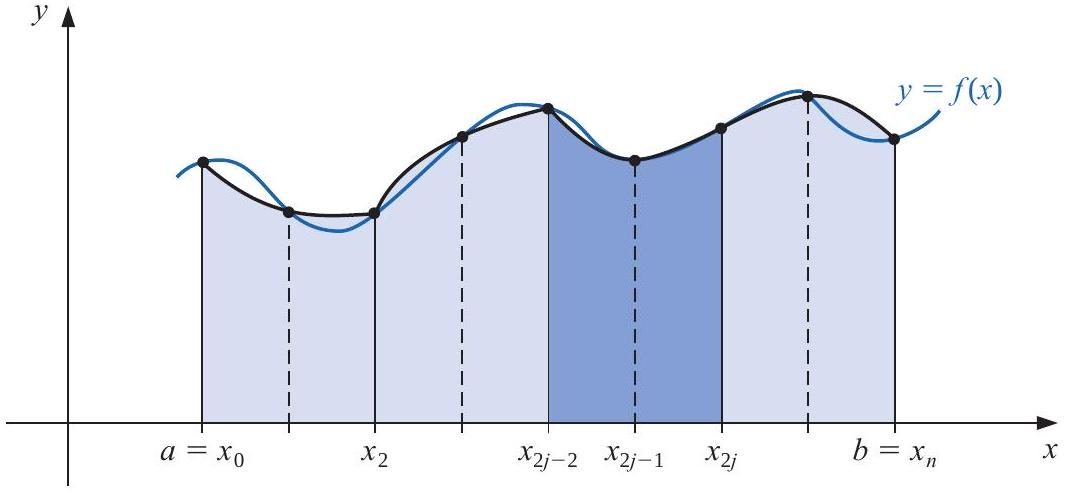
\includegraphics[width=12cm]{2025_05_15_85b7f7df47271a498e1dg-32.JPG}
\caption{\scriptsize Figure $1$}
\label{fig:2025_05_15_85b7f7df47271a498e1dg-32}
\end{figure}

With $h=(b-a) / n$ and $x_{j}=a+j h$, for each $j=0,1, \ldots, n$, we have

$$
\begin{aligned}
\int_{a}^{b} f(x) d x & =\sum_{j=1}^{n / 2} \int_{x_{2 j-2}}^{x_{2 j}} f(x) d x \\
& =\sum_{j=1}^{n / 2}\left\{\frac{h}{3}\left[f\left(x_{2 j-2}\right)+4 f\left(x_{2 j-1}\right)+f\left(x_{2 j}\right)\right]-\frac{h^{5}}{90} f^{(4)}\left(\xi_{j}\right)\right\}
\end{aligned}
$$

for some $\xi_{j}$ with $x_{2 j-2}<\xi_{j}<x_{2 j}$, provided that $f \in C^{4}[a, b]$. Using the fact that for each $j=1,2, \ldots,(n / 2)-1$ we have $f\left(x_{2 j}\right)$ appearing in the term corresponding to the interval $\left[x_{2 j-2}, x_{2 j}\right]$ and also in the term corresponding to the interval $\left[x_{2 j}, x_{2 j+2}\right]$, we can reduce this sum to

$$
\int_{a}^{b} f(x) d x=\frac{h}{3}\left[f\left(x_{0}\right)+2 \sum_{j=1}^{(n / 2)-1} f\left(x_{2 j}\right)+4 \sum_{j=1}^{n / 2} f\left(x_{2 j-1}\right)+f\left(x_{n}\right)\right]-\frac{h^{5}}{90} \sum_{j=1}^{n / 2} f^{(4)}\left(\xi_{j}\right)
$$

The error associated with this approximation is

$$
E(f)=-\frac{h^{5}}{90} \sum_{j=1}^{n / 2} f^{(4)}\left(\xi_{j}\right)
$$

where $x_{2 j-2}<\xi_{j}<x_{2 j}$, for each $j=1,2, \ldots, n / 2$.

%If $f \in C^{4}[a, b]$, the Extreme Value Theorem implies that $f^{(4)}$ assumes its maximum and minimum in $[a, b]$. Since
%
%$$
%\min _{x \in[a, b]} f^{(4)}(x) \leq f^{(4)}\left(\xi_{j}\right) \leq \max _{x \in[a, b]} f^{(4)}(x)
%$$
%
%we have
%
%$$
%\frac{n}{2} \min _{x \in[a, b]} f^{(4)}(x) \leq \sum_{j=1}^{n / 2} f^{(4)}\left(\xi_{j}\right) \leq \frac{n}{2} \max _{x \in[a, b]} f^{(4)}(x)
%$$
%
%and
%
%$$
%\min _{x \in[a, b]} f^{(4)}(x) \leq \frac{2}{n} \sum_{j=1}^{n / 2} f^{(4)}\left(\xi_{j}\right) \leq \max _{x \in[a, b]} f^{(4)}(x)
%$$
%
%By the Intermediate Value Theorem 1.11, there is a $\mu \in(a, b)$ such that
%
%$$
%f^{(4)}(\mu)=\frac{2}{n} \sum_{j=1}^{n / 2} f^{(4)}\left(\xi_{j}\right)
%$$
%
%Thus
%
%$$
%E(f)=-\frac{h^{5}}{90} \sum_{j=1}^{n / 2} f^{(4)}\left(\xi_{j}\right)=-\frac{h^{5}}{180} n f^{(4)}(\mu)
%$$
%
%or, since $h=(b-a) / n$,
%
%$$
%E(f)=-\frac{(b-a)}{180} h^{4} f^{(4)}(\mu)
%$$

These observations produce the following result.

\begin{theorem}
Let $f \in C^{4}[a, b], n$ be even, $h=(b-a) / n$, and $x_{j}=a+j h$, for each $j=0,1, \ldots, n$. There exists a $\mu \in(a, b)$ for which the Composite Simpson's rule for $n$ subintervals can be written with its error term as

$$
\int_{a}^{b} f(x) d x=\frac{h}{3}\left[f(a)+2 \sum_{j=1}^{(n / 2)-1} f\left(x_{2 j}\right)+4 \sum_{j=1}^{n / 2} f\left(x_{2 j-1}\right)+f(b)\right]-\frac{b-a}{180} h^{4} f^{(4)}(\mu)
$$
\end{theorem}
Notice that the error term for the Composite Simpson's rule is $O\left(h^{4}\right)$, whereas it was $O\left(h^{5}\right)$ for the standard Simpson's rule. However, these rates are not comparable because for standard Simpson's rule we have $h$ fixed at $h=(b-a) / 2$, but for Composite Simpson's rule we have $h=(b-a) / n$, for $n$ an even integer. This permits us to considerably reduce the value of $h$ when the Composite Simpson's rule is used.
%
%Algorithm 4.1 uses the Composite Simpson's rule on $n$ subintervals. This is the most frequently used general-purpose quadrature algorithm.
%
%\section*{Composite Simpson's Rule}
%To approximate the integral $I=\int_{a}^{b} f(x) d x$ :\\
%INPUT endpoints $a, b$; even positive integer $n$.\\
%OUTPUT approximation $X I$ to $I$.\\
%Step 1 Set $h=(b-a) / n$.\\
%Step 2 Set XIO $=f(a)+f(b)$;\\
%XI1 $=0 ; \quad$ (Summation of $\left.f\left(x_{2 i-1}\right).\right)$\\
%XI2 $=0 . \quad$ (Summation of $f\left(x_{2 i}\right)$. )\\
%Step 3 For $i=1, \ldots, n-1$ do Steps 4 and 5.\\
%Step 4 Set $X=a+i h$.\\
%Step 5 If $i$ is even then set $X I 2=X I 2+f(X)$\\
%else set $X I 1=X I 1+f(X)$.\\
%Step 6 Set $X I=h(X I 0+2 \cdot X I 2+4 \cdot X I 1) / 3$.\\
%Step 7 OUTPUT (XI);\\
%STOP.

The subdivision approach can be applied to any of the Newton-Cotes formulas. The extensions of the Trapezoidal (see Figure 4.8) and Midpoint rules are given without proof. The Trapezoidal rule requires only one interval for each application, so the integer $n$ can be either odd or even.

\begin{theorem}
Let $f \in C^{2}[a, b], h=(b-a) / n$, and $x_{j}=a+j h$, for each $j=0,1, \ldots, n$. There exists a $\mu \in(a, b)$ for which the {\bf Composite Trapezoidal rule} for $n$ subintervals can be written with its error term as

$$
\int_{a}^{b} f(x) d x=\frac{h}{2}\left[f(a)+2 \sum_{j=1}^{n-1} f\left(x_{j}\right)+f(b)\right]-\frac{b-a}{12} h^{2} f^{\prime \prime}(\mu)
$$
\end{theorem}

\newpage
\begin{figure}[h]
\centering
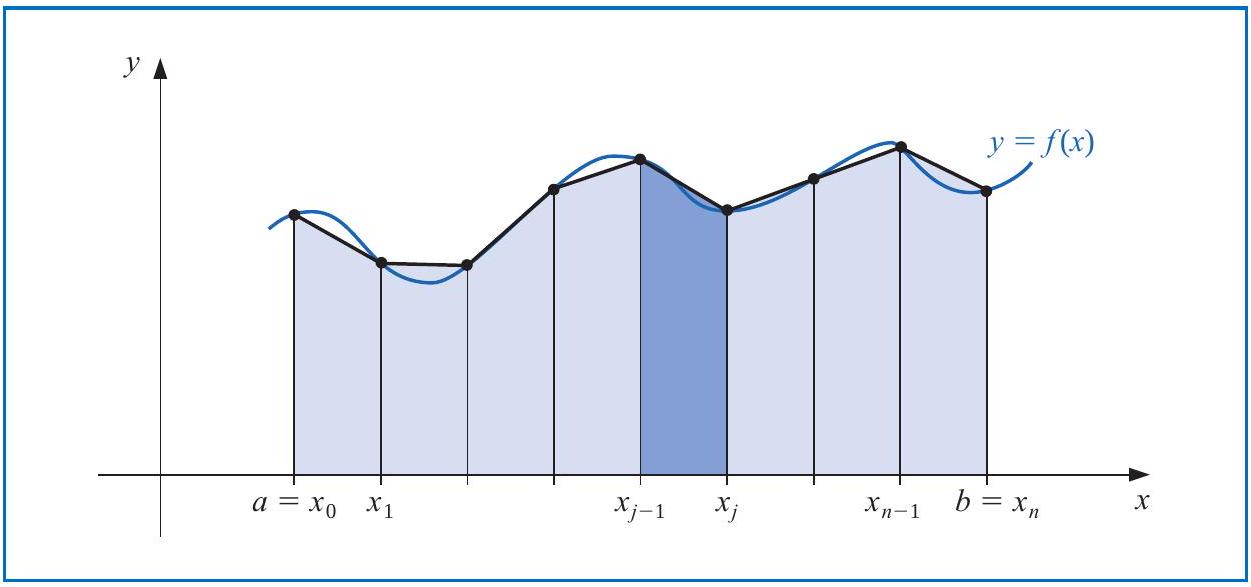
\includegraphics[width=12cm]{2025_05_15_85b7f7df47271a498e1dg-35(1)}
\caption{\scriptsize Figure $2$}
\label{fig:2025_05_15_85b7f7df47271a498e1dg-35(1)}
\end{figure}

For the Composite Midpoint rule, $n$ must again be even. (See Figure \ref{fig:2025_05_15_85b7f7df47271a498e1dg-35}.)

\begin{figure}[h]
\centering
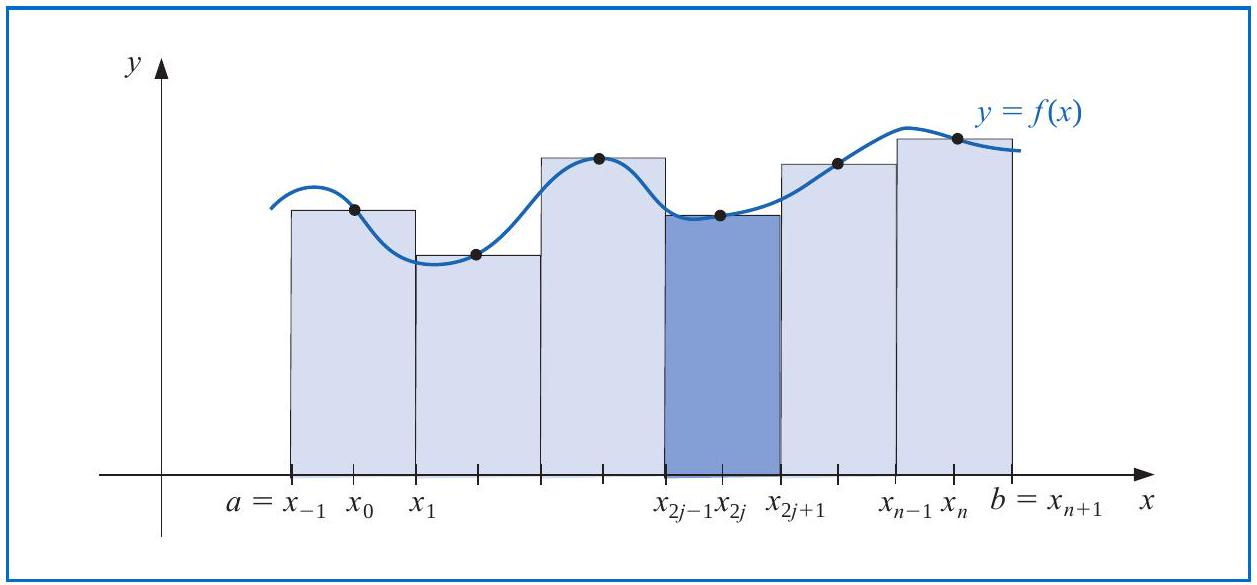
\includegraphics[width=12cm]{2025_05_15_85b7f7df47271a498e1dg-35}
\caption{\scriptsize Figure $3$}
\label{fig:2025_05_15_85b7f7df47271a498e1dg-35}
\end{figure}


\begin{theorem}
Let $f \in C^{2}[a, b], n$ be even, $h=(b-a) /(n+2)$, and $x_{j}=a+(j+1) h$ for each $j=-1,0, \ldots, n+1$. There exists a $\mu \in(a, b)$ for which the Composite Midpoint rule for $n+2$ subintervals can be written with its error term as

$$
\int_{a}^{b} f(x) d x=2 h \sum_{j=0}^{n / 2} f\left(x_{2 j}\right)+\frac{b-a}{6} h^{2} f^{\prime \prime}(\mu)
$$
\end{theorem}

\begin{example}
Determine values of $h$ that will ensure an approximation error of less than 0.00002 when approximating $\int_{0}^{\pi} \sin x d x$ and employing\\
(a) Composite Trapezoidal rule and (b) Composite Simpson's rule.
\end{example}

\begin{mysolution}
\begin{enumerate}[label=(\alph*)]
\item The error form for the Composite Trapezoidal rule for $f(x)=\sin x$ on $[0, \pi]$ is

$$
\left|\frac{\pi h^{2}}{12} f^{\prime \prime}(\mu)\right|=\left|\frac{\pi h^{2}}{12}(-\sin \mu)\right|=\frac{\pi h^{2}}{12}|\sin \mu| .
$$

To ensure sufficient accuracy with this technique we need to have

$$
\frac{\pi h^{2}}{12}|\sin \mu| \leq \frac{\pi h^{2}}{12}<0.00002
$$

Since $h=\pi / n$ implies that $n=\pi / h$, we need

$$
\frac{\pi^{3}}{12 n^{2}}<0.00002 \quad \text { which implies that } n>\left(\frac{\pi^{3}}{12(0.00002)}\right)^{1 / 2} \approx 359.44
$$

and the Composite Trapezoidal rule requires $n \geq 360$.
\item The error form for the Composite Simpson's rule for $f(x)=\sin x$ on $[0, \pi]$ is

$$
\left|\frac{\pi h^{4}}{180} f^{(4)}(\mu)\right|=\left|\frac{\pi h^{4}}{180} \sin \mu\right|=\frac{\pi h^{4}}{180}|\sin \mu| .
$$

To ensure sufficient accuracy with this technique we need to have

$$
\frac{\pi h^{4}}{180}|\sin \mu| \leq \frac{\pi h^{4}}{180}<0.00002
$$

Using again the fact that $n=\pi / h$ gives

$$
\frac{\pi^{5}}{180 n^{4}}<0.00002 \quad \text { which implies that } \quad n>\left(\frac{\pi^{5}}{180(0.00002)}\right)^{1 / 4} \approx 17.07
$$

So Composite Simpson's rule requires only $n \geq 18$.\\
Composite Simpson's rule with $n=18$ gives

$$
\int_{0}^{\pi} \sin x d x \approx \frac{\pi}{54}\left[2 \sum_{j=1}^{8} \sin \left(\frac{j \pi}{9}\right)+4 \sum_{j=1}^{9} \sin \left(\frac{(2 j-1) \pi}{18}\right)\right]=2.0000104
$$

This is accurate to within about $10^{-5}$ because the true value is $-\cos (\pi)-(-\cos (0))=2$.
\end{enumerate}\qed
\end{mysolution}

Composite Simpson's rule is the clear choice if you wish to minimize computation. For comparison purposes, consider the Composite Trapezoidal rule using $h=\pi / 18$ for the integral in Example 2. This approximation uses the same function evaluations as Composite Simpson's rule but the approximation in this case\\
$\int_{0}^{\pi} \sin x d x \approx \frac{\pi}{36}\left[2 \sum_{j=1}^{17} \sin \left(\frac{j \pi}{18}\right)+\sin 0+\sin \pi\right]=\frac{\pi}{36}\left[2 \sum_{j=1}^{17} \sin \left(\frac{j \pi}{18}\right)\right]=1.9949205$.\\
is accurate only to about $5 \times 10^{-3}$.\\
%Maple contains numerous procedures for numerical integration in the NumericalAnalysis subpackage of the Student package. First access the library as usual with\\[0pt]
%with(Student[NumericalAnalysis])\\
%The command for all methods is Quadrature with the options in the call specifying the method to be used. We will use the Trapezoidal method to illustrate the procedure. First define the function and the interval of integration with\\
%$f:=x \rightarrow \sin (x) ; a:=0.0 ; b:=\pi$
%
%Numerical integration is expected to be stable, whereas numerical differentiation is unstable.
%
%After Maple responds with the function and the interval, enter the command\\
%Quadrature $(f(x), x=$ a.. $b$, method $=$ trapezoid, partition $=20$, output $=$ value $)$\\
%1.995885973
%
%The value of the step size $h$ in this instance is the width of the interval $b-a$ divided by the number specified by partition $=20$.
%
%Simpson's method can be called in a similar manner, except that the step size $h$ is determined by $b-a$ divided by twice the value of partition. Hence, the Simpson's rule approximation using the same nodes as those in the Trapezoidal rule is called with
%
%Quadrature $(f(x), x=a . . b$, method $=$ simpson,partition $=10$, output $=$ value $)$\\
%2.000006785
%
%Any of the Newton-Cotes methods can be called using the option
%
%$$
%\text { method }=\text { newtoncotes }[\text { open }, n] \text { or } \text { method }=\text { newtoncotes }[\text { closed }, n]
%$$
%
%Be careful to correctly specify the number in partition when an even number of divisions is required, and when an open method is employed.
%
\subsection*{Round-Off Error Stability}
In Example 2 we saw that ensuring an accuracy of $2 \times 10^{-5}$ for approximating $\int_{0}^{\pi} \sin x d x$ required $360$ subdivisions of $[0, \pi]$ for the Composite Trapezoidal rule and only $18$ for Composite Simpson's rule. In addition to the fact that less computation is needed for the Simpson's technique, you might suspect that because of fewer computations this method would also involve less round-off error. However, an important property shared by all the composite integration techniques is a stability with respect to round-off error. That is, the round-off error does not depend on the number of calculations performed.

To demonstrate this rather amazing fact, suppose we apply the Composite Simpson's rule with $n$ subintervals to a function $f$ on $[a, b]$ and determine the maximum bound for the round-off error. Assume that $f\left(x_{i}\right)$ is approximated by $\tilde{f}\left(x_{i}\right)$ and that

$$
f\left(x_{i}\right)=\tilde{f}\left(x_{i}\right)+e_{i}, \quad \text { for each } i=0,1, \ldots, n,
$$

where $e_{i}$ denotes the round-off error associated with using $\tilde{f}\left(x_{i}\right)$ to approximate $f\left(x_{i}\right)$. Then the accumulated error, $e(h)$, in the Composite Simpson's rule is

$$
\begin{aligned}
e(h) & =\left|\frac{h}{3}\left[e_{0}+2 \sum_{j=1}^{(n / 2)-1} e_{2 j}+4 \sum_{j=1}^{n / 2} e_{2 j-1}+e_{n}\right]\right| \\
& \leq \frac{h}{3}\left[\left|e_{0}\right|+2 \sum_{j=1}^{(n / 2)-1}\left|e_{2 j}\right|+4 \sum_{j=1}^{n / 2}\left|e_{2 j-1}\right|+\left|e_{n}\right|\right] .
\end{aligned}
$$

If the round-off errors are uniformly bounded by $\varepsilon$, then

$$
e(h) \leq \frac{h}{3}\left[\varepsilon+2\left(\frac{n}{2}-1\right) \varepsilon+4\left(\frac{n}{2}\right) \varepsilon+\varepsilon\right]=\frac{h}{3} 3 n \varepsilon=n h \varepsilon .
$$

But $n h=b-a$, so

$$
e(h) \leq(b-a) \varepsilon
$$

a bound independent of $h$ (and $n$ ). This means that, even though we may need to divide an interval into more parts to ensure accuracy, the increased computation that is required does not increase the round-off error. This result implies that the procedure is stable as $h$ approaches zero. Recall that this was not true of the numerical differentiation procedures we have considered.

\begin{myexercise}%\label{Comprehensionquiz2}
Approximate the integral $\int_{-2}^{2} x^{3} e^{x} d x, \quad n=4$
\begin{enumerate}[label=(\alph*)]
\item Composite Trapezoidal rule with the indicated values of $n$
\item Composite Simpson's rule with the indicated values of $n$
\item Composite Midpoint rule with $n+2$ subintervals.
\end{enumerate}

\begin{mysolution}
\begin{multicols}{3}
\begin{enumerate}[label=(\alph*)]
\item $31.3653$
\item $22.47713$
\item $11.1568$
\end{enumerate}
\end{multicols}
\end{mysolution}
\end{myexercise}

\section{Romberg Integration}

\begin{youtube}
This video presents a discussion on Romberg integration. Follow the discussion and then solve the problems in the subsequent quiz.
\mylink{https://www.youtube.com/watch?v=oAh0qTJtSuk}
\end{youtube}


\begin{myexercise}%\label{Comprehensionquiz2}
Use Romberg integration to compute $R_{3,3}$ for the following integrals.
\begin{multicols}{2}
\begin{enumerate}[label=(\alph*)]
\item  $\quad \int_{1}^{1.5} x^{2} \ln x d x$\\
\item $\int_{0}^{1} x^{2} e^{-x} d x$\\
\item $\quad \int_{0}^{0.35} \frac{2}{x^{2}-4} d x$\\
\item $\quad \int_{0}^{\pi / 4} x^{2} \sin x d x$\\
\item $\quad \int_{0}^{\pi / 4} e^{3 x} \sin 2 x d x$\\
\item $\quad \int_{1}^{1.6} \frac{2 x}{x^{2}-4} d x$\\
\item $\quad \int_{3}^{3.5} \frac{x}{\sqrt{x^{2}-4}} d x$\\
\item $\int_{0}^{\pi / 4}(\cos x)^{2} d x$
\end{enumerate}
\end{multicols}
\begin{mysolution}
\begin{multicols}{2}
\begin{enumerate}[label=(\alph*)]
\item $0.1922593$ \item $0.1606105$ \item $-0.1768200$ \item $0.08875677$ \item $2.5879685$ \item $-0.7341567$ \item $0.6362135$ \item $0.6426970$
\end{enumerate}
\end{multicols}
\end{mysolution}
\end{myexercise}



\section{Adaptive Quadrature Methods}
%\activities
%Read on adaptive quadrature methods in pages \textcolor{red}{\bf page $220-227$} of the following reference and then attempt the subsequent quiz
%\begin{activity}[\cg Reading]
%\begin{enumerate}
%\item Burden, R. L., Faires, J. D., Burden, A. M. (2015). Numerical Analysis. Tenth Edition, Cengage Learning.\\
%\end{enumerate}
%\end{activity}
\activities
Read on adaptive quadrature method in the reference provided in the link below in the pages Appendix C3 and then attempt the subsequent quiz.
\begin{activity}[\cg Reading]
%\begin{enumerate}
%\item \mylink{https://math.libretexts.org/Bookshelves/Calculus/CLP-2\_Integral\_Calculus\_(Feldman\_Rechnitzer\_and\_Yeager)/04\%3A\_Appendices/4.03\%3A\_C\%3A\_More\_About\_Numerical\_Integration/4.3.01\%3A\_C.1\%3A\_Richardson\_Extrapolation}
%\end{enumerate}
\mylink{https://math.libretexts.org/Bookshelves/Calculus/\\CLP-2\_Integral\_Calculus\_(Feldman\_Rechnitzer\_and\_Yeager)}
\end{activity}
\begin{myexercise}%\label{Comprehensionquiz2}
Compute the Simpson's rule approximations $S(a, b), S(a,(a+b) / 2)$, and $S((a+b) / 2, b)$ for the following integrals, and verify the estimate given in the approximation formula.
\begin{multicols}{2}
\begin{enumerate}[label=(\alph*)]
\item $\int_1^{1.5}x^2\ln x\, dx$
\item $\int_{0}^{1} x^{2} e^{-x} d x$
\item $\int_{0}^{0.35} \frac{2}{x^{2}-4} d x$
\item $\int_{0}^{\pi / 4} x^{2} \sin x d x$
%\item $\int_{0}^{\pi / 4} e^{3 x} \sin 2 x d x$
%\item $\int_{1}^{1.6} \frac{2 x}{x^{2}-4} d x$
%\item $\int_{3}^{3.5} \frac{x}{\sqrt{x^{2}-4}} d x$
%\item $\int_{0}^{\pi / 4}(\cos x)^{2} d x$
\end{enumerate}
\end{multicols}

\begin{mysolution}
\begin{enumerate}[label=(\alph*)]
\item $S(1,1.5)=0.19224530$, $S(1,1.25)=0.039372434$, $S(1.25,1.5)=0.15288602$, and the actual value is $0.19225935$.
\item $S(0,1)=0.16240168$, $S(0,0.5)=0.028861071$, $S(0.5,1)=0.13186140$, and the actual value is $0.16060279$.
\item $S(0,0.35)=-0.17682156$, $S(0,0.175)=-0.087724382$, $S(0.175,0.35)=-0.089095736$, and the actual value is $-0.17682002$.
\item $S\left(0,\frac{\pi}{4}\right)=0.087995669$, $S\left(0,\frac{\pi}{8}\right)=0.0058315797$, $S\left(\frac{\pi}{8},\frac{\pi}{4}\right)=0.082877624$, and the actual value is $0.088755285$.
%\item $S\left(0,\frac{\pi}{4}\right)=2.5836964$, $S\left(0,\frac{\pi}{8}\right)=0.33088926$, $S\left(\frac{\pi}{8},\frac{\pi}{4}\right)=2.2568121$, and the actual value is $2.5886286$.
%\item $S(1,1.6)=-0.73910533$, $S(1,1.3)=-0.26141244$, $S(1.3,1.6)=-0.47305351$, and the actual value is $-0.73396917$.
%\item $S(3,3.5)=0.63623873$, $S(3,3.25)=0.32567095$, $S(3.25,3.5)=0.31054412$, and the actual value is $0.63621334$.
%\item $S\left(0,\frac{\pi}{4}\right)=0.64326905$, $S\left(0,\frac{\pi}{8}\right)=0.37315002$, $S\left(\frac{\pi}{8},\frac{\pi}{4}\right)=0.26958270$, and the actual value is $0.64269908$.
\end{enumerate}
\end{mysolution}
\end{myexercise}

\section{Gaussian Quadrature}
\videolesson
\begin{selfvideo}[2]
%LESSON 3: 
This video presents a discussion on Gaussian quadrature. Follow the discussion and then solve the problems in the subsequent quiz.
\end{selfvideo}
%\begin{boxB}Question: \end{boxB}

The Newton-Cotes formulas in Section $4$ of Module $4$ were derived by integrating interpolating polynomials. The error term in the interpolating polynomial of degree $n$ involves the $(n+1)$ st derivative of the function being approximated, so a Newton-Cotes formula is exact when approximating the integral of any polynomial of degree less than or equal to $n$.

All the Newton-Cotes formulas use values of the function at equally-spaced points. This restriction is convenient when the formulas are combined to form the composite rules we considered in Section $1$ of this Module, but it can significantly decrease the accuracy of the approximation. Consider, for example, the Trapezoidal rule applied to determine the integrals of the functions whose graphs are shown in Figure \ref{fig:2025_05_15_85b7f7df47271a498e1dg-57}.

%Figure 4.15\\
\begin{figure}[h]
\centering
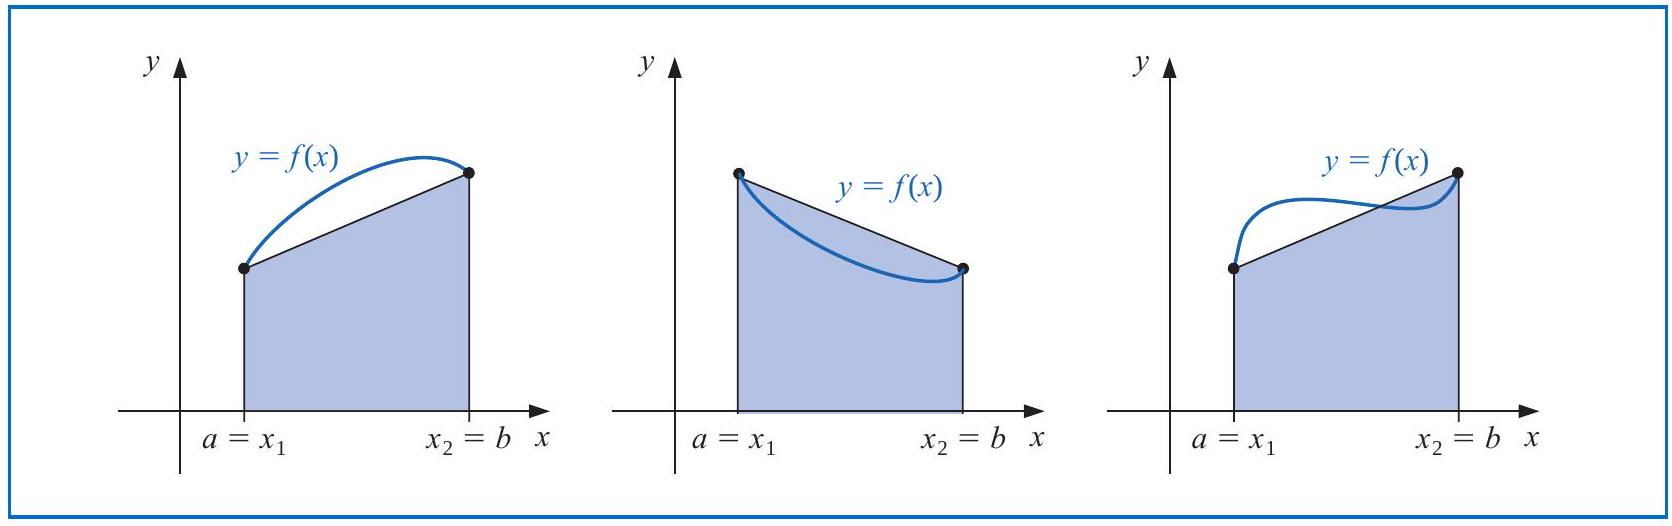
\includegraphics[width=15cm]{2025_05_15_85b7f7df47271a498e1dg-57}
\caption{\scriptsize Figure $4$}
\label{fig:2025_05_15_85b7f7df47271a498e1dg-57}
\end{figure}

The Trapezoidal rule approximates the integral of the function by integrating the linear function that joins the endpoints of the graph of the function. But this is not likely the best line for approximating the integral. Lines such as those shown in Figure \ref{fig:2025_05_15_85b7f7df47271a498e1dg-57(1)} would likely give much better approximations in most cases.

%Figure 4.16\\
\begin{figure}[h]
\centering
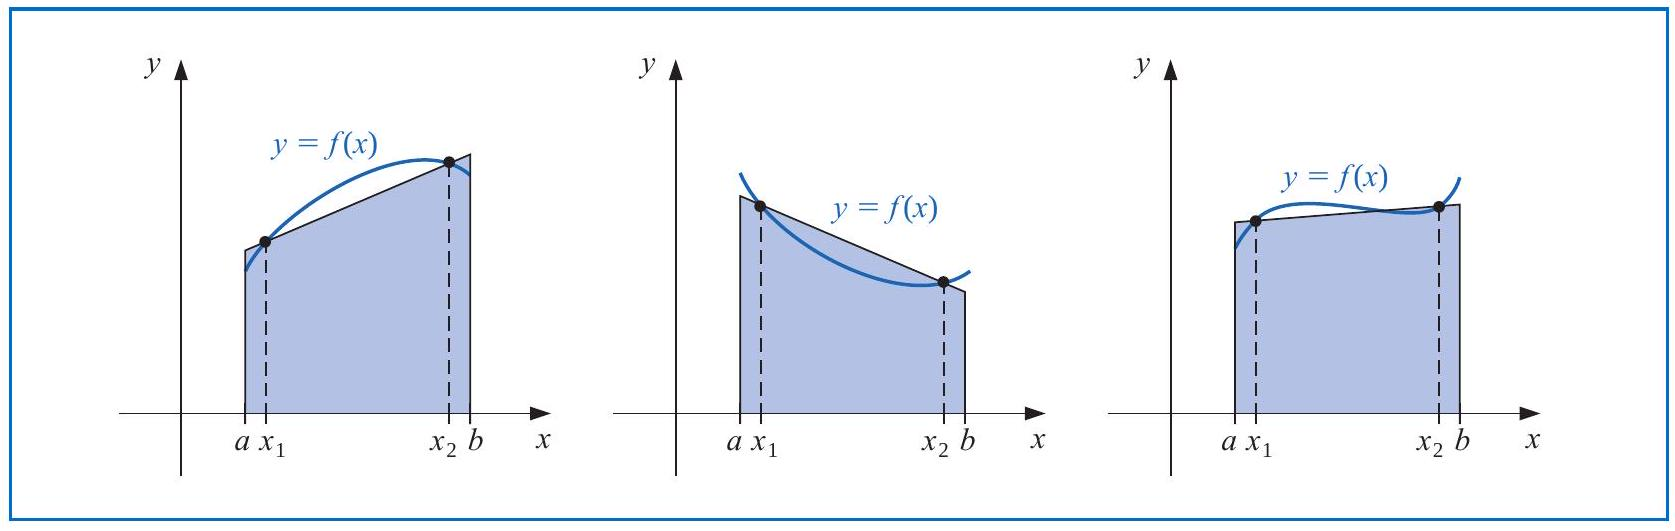
\includegraphics[width=15cm]{2025_05_15_85b7f7df47271a498e1dg-57(1)}
\caption{\scriptsize Figure $5$}
\label{fig:2025_05_15_85b7f7df47271a498e1dg-57(1)}
\end{figure}

%Gauss demonstrated his method of efficient numerical integration in a paper that was presented to the Göttingen Society in 1814. He let the nodes as well as the coefficients of the function evaluations be parameters in the summation formula and found the optimal placement of the nodes. Goldstine [Golds], pp 224-232, has an interesting description of his development.

Gaussian quadrature chooses the points for evaluation in an optimal, rather than equally spaced, way. The nodes $x_{1}, x_{2}, \ldots, x_{n}$ in the interval $[a, b]$ and coefficients $c_{1}, c_{2}, \ldots, c_{n}$, are chosen to minimize the expected error obtained in the approximation

$$
\int_{a}^{b} f(x) d x \approx \sum_{i=1}^{n} c_{i} f\left(x_{i}\right)
$$

To measure this accuracy, we assume that the best choice of these values produces the exact result for the largest class of polynomials, that is, the choice that gives the greatest degree of precision.

The coefficients $c_{1}, c_{2}, \ldots, c_{n}$ in the approximation formula are arbitrary, and the nodes $x_{1}, x_{2}, \ldots, x_{n}$ are restricted only by the fact that they must lie in $[a, b]$, the interval of integration. This gives us $2 n$ parameters to choose. If the coefficients of a polynomial are\\
considered parameters, the class of polynomials of degree at most $2 n-1$ also contains $2 n$ parameters. This, then, is the largest class of polynomials for which it is reasonable to expect a formula to be exact. With the proper choice of the values and constants, exactness on this set can be obtained.

To illustrate the procedure for choosing the appropriate parameters, we will show how to select the coefficients and nodes when $n=2$ and the interval of integration is $[-1,1]$. We will then discuss the more general situation for an arbitrary choice of nodes and coefficients and show how the technique is modified when integrating over an arbitrary interval.

Suppose we want to determine $c_{1}, c_{2}, x_{1}$, and $x_{2}$ so that the integration formula

$$
\int_{-1}^{1} f(x) d x \approx c_{1} f\left(x_{1}\right)+c_{2} f\left(x_{2}\right)
$$

gives the exact result whenever $f(x)$ is a polynomial of degree $2(2)-1=3$ or less, that is, when

$$
f(x)=a_{0}+a_{1} x+a_{2} x^{2}+a_{3} x^{3}
$$

for some collection of constants, $a_{0}, a_{1}, a_{2}$, and $a_{3}$. Because

$$
\int\left(a_{0}+a_{1} x+a_{2} x^{2}+a_{3} x^{3}\right) d x=a_{0} \int 1 d x+a_{1} \int x d x+a_{2} \int x^{2} d x+a_{3} \int x^{3} d x
$$

this is equivalent to showing that the formula gives exact results when $f(x)$ is $1, x, x^{2}$, and $x^{3}$. Hence, we need $c_{1}, c_{2}, x_{1}$, and $x_{2}$, so that

$$
\begin{array}{cc}
c_{1} \cdot 1+c_{2} \cdot 1=\int_{-1}^{1} 1 d x=2, & c_{1} \cdot x_{1}+c_{2} \cdot x_{2}=\int_{-1}^{1} x d x=0 \\
c_{1} \cdot x_{1}^{2}+c_{2} \cdot x_{2}^{2}=\int_{-1}^{1} x^{2} d x=\frac{2}{3}, & \text { and } \\
c_{1} \cdot x_{1}^{3}+c_{2} \cdot x_{2}^{3}=\int_{-1}^{1} x^{3} d x=0
\end{array}
$$

A little algebra shows that this system of equations has the unique solution

$$
c_{1}=1, \quad c_{2}=1, \quad x_{1}=-\frac{\sqrt{3}}{3}, \quad \text { and } \quad x_{2}=\frac{\sqrt{3}}{3},
$$

which gives the approximation formula


\begin{equation}\label{eqngaussquad1}
\int_{-1}^{1} f(x) d x \approx f\left(\frac{-\sqrt{3}}{3}\right)+f\left(\frac{\sqrt{3}}{3}\right) \tag{4.40}
\end{equation}


This formula has degree of precision 3, that is, it produces the exact result for every polynomial of degree 3 or less.

\subsection*{Legendre Polynomials}
The technique we have described could be used to determine the nodes and coefficients for formulas that give exact results for higher-degree polynomials, but an alternative method obtains them more easily. The set that is relevant to our problem is the Legendre polynomials, a collection $\left\{P_{0}(x), P_{1}(x), \ldots, P_{n}(x), \ldots,\right\}$ with properties:\\
\begin{enumerate}[label=(\arabic*)]
\item For each $n, P_{n}(x)$ is a monic polynomial of degree $n$.

Recall that monic polynomials have leading coefficient 1.

%Adrien-Marie Legendre (1752-1833) introduced this set of polynomials in 1785. He had numerous priority disputes with Gauss, primarily due to Gauss' failure to publish many of his original results until long after he had discovered them.
\item $\displaystyle\int_{-1}^1P(x)P_n(x)\,dx=0$ whenever $P(x)$ is a polynomial of degree less than $n$.
\end{enumerate}

The first few Legendre polynomials are
\[P_0(x)=1,\quad P_1(x)=x,\quad P_2(x)=x^2-\frac13,\]
\[P_3(x)=x^3-\frac35x,\quad\mbox{ and } \quad P_4(x)=x^4-\frac67x^2+ \frac{3}{35}.\]
 The roots of these polynomials are distinct, lie in the interval $(-1,1)$, have a symmetry with respect to the origin, and, most importantly, are the correct choice for determining the parameters that give us the nodes and coefficients for our quadrature method.

The nodes $x_1, x_2, \ldots, x_n$ needed to produce an integral approximation formula that gives exact results for any polynomial of degree less than $2n$ are the roots of the $nth-$degree Legendre polynomial. This is established by the following result.

\begin{theorem}\label{thm:Legendpolythm1}
Suppose that $x_{1}, x_{2}, \ldots, x_{n}$ are the roots of the $n$th Legendre polynomial $P_{n}(x)$ and that for each $i=1,2, \ldots, n$, the numbers $c_{i}$ are defined by

$$
c_{i}=\int_{-1}^{1} \prod_{\substack{j=1 \\ j \neq i}}^{n} \frac{x-x_{j}}{x_{i}-x_{j}} d x
$$

If $P(x)$ is any polynomial of degree less than $2 n$, then

$$
\int_{-1}^{1} P(x) d x=\sum_{i=1}^{n} c_{i} P\left(x_{i}\right)
$$
\end{theorem}
%
%Proof Let us first consider the situation for a polynomial $P(x)$ of degree less than $n$. Rewrite $P(x)$ in terms of $(n-1)$ st Lagrange coefficient polynomials with nodes at the roots of the $n$th Legendre polynomial $P_{n}(x)$. The error term for this representation involves the $n$th derivative of $P(x)$. Since $P(x)$ is of degree less than $n$, the $n$th derivative of $P(x)$ is 0 , and this representation of is exact. So
%
%$$
%P(x)=\sum_{i=1}^{n} P\left(x_{i}\right) L_{i}(x)=\sum_{i=1}^{n} \prod_{\substack{j=1 \\ j \neq i}}^{n} \frac{x-x_{j}}{x_{i}-x_{j}} P\left(x_{i}\right)
%$$
%
%and
%
%$$
%\begin{aligned}
%\int_{-1}^{1} P(x) d x & =\int_{-1}^{1}\left[\sum_{i=1}^{n} \prod_{\substack{j=1 \\
%j \neq i}}^{n} \frac{x-x_{j}}{x_{i}-x_{j}} P\left(x_{i}\right)\right] d x \\
%& =\sum_{i=1}^{n}\left[\int_{-1}^{1} \prod_{\substack{j=1 \\
%j \neq i}}^{n} \frac{x-x_{j}}{x_{i}-x_{j}} d x\right] P\left(x_{i}\right)=\sum_{i=1}^{n} c_{i} P\left(x_{i}\right)
%\end{aligned}
%$$
%
%Hence the result is true for polynomials of degree less than $n$.\\
%Now consider a polynomial $P(x)$ of degree at least $n$ but less than $2 n$. Divide $P(x)$ by the $n$th Legendre polynomial $P_{n}(x)$. This gives two polynomials $Q(x)$ and $R(x)$, each of degree less than $n$, with
%
%$$
%P(x)=Q(x) P_{n}(x)+R(x)
%$$
%
%Note that $x_{i}$ is a root of $P_{n}(x)$ for each $i=1,2, \ldots, n$, so we have
%
%$$
%P\left(x_{i}\right)=Q\left(x_{i}\right) P_{n}\left(x_{i}\right)+R\left(x_{i}\right)=R\left(x_{i}\right) .
%$$
%
%We now invoke the unique power of the Legendre polynomials. First, the degree of the polynomial $Q(x)$ is less than $n$, so (by Legendre property (2)),
%
%$$
%\int_{-1}^{1} Q(x) P_{n}(x) d x=0
%$$
%
%Then, since $R(x)$ is a polynomial of degree less than $n$, the opening argument implies that
%
%$$
%\int_{-1}^{1} R(x) d x=\sum_{i=1}^{n} c_{i} R\left(x_{i}\right)
%$$
%
%Putting these facts together verifies that the formula is exact for the polynomial $P(x)$ :
%
%$$
%\int_{-1}^{1} P(x) d x=\int_{-1}^{1}\left[Q(x) P_{n}(x)+R(x)\right] d x=\int_{-1}^{1} R(x) d x=\sum_{i=1}^{n} c_{i} R\left(x_{i}\right)=\sum_{i=1}^{n} c_{i} P\left(x_{i}\right)
%$$
%
The constants $c_{i}$ needed for the quadrature rule can be generated from the equation in Theorem \ref{thm:Legendpolythm1}, but both these constants and the roots of the Legendre polynomials are extensively tabulated. Table \ref{legendpolytable1} lists these values for $n=2,3,4$, and 5 .

%\newpage
\begin{table}[h]
\centering
\begin{tabular}{|l|l|l|}
\hline
$n$ & Roots $r_{n, i}$ & Coefficients $c_{n, i}$ \\
\hline
\multirow[t]{2}{*}{2} & 0.5773502692 & 1.0000000000 \\
\hline
 & -0.5773502692 & 1.0000000000 \\
\hline
\multirow[t]{3}{*}{3} & 0.7745966692 & 0.555555556 \\
\hline
 & 0.0000000000 & 0.888888889 \\
\hline
 & -0.7745966692 & 0.555555556 \\
\hline
\multirow[t]{4}{*}{4} & 0.8611363116 & 0.3478548451 \\
\hline
 & 0.3399810436 & 0.6521451549 \\
\hline
 & -0.3399810436 & 0.6521451549 \\
\hline
 & -0.8611363116 & 0.3478548451 \\
\hline
\multirow[t]{5}{*}{5} & 0.9061798459 & 0.2369268850 \\
\hline
 & 0.5384693101 & 0.4786286705 \\
\hline
 & 0.0000000000 & 0.5688888889 \\
\hline
 & -0.5384693101 & 0.4786286705 \\
\hline
 & -0.9061798459 & 0.2369268850 \\
\hline
\end{tabular}
\caption{\scriptsize Table $1$}
\label{legendpolytable1}
\end{table}

\begin{example}
Approximate $\int_{-1}^{1} e^{x} \cos x d x$ using Gaussian quadrature with $n=3$.
\end{example}

\begin{mysolution}
The entries in Table \ref{legendpolytable1} give us

$$
\begin{aligned}
\int_{-1}^{1} e^{x} \cos x d x \approx & 0 . \overline{5} e^{0.774596692} \cos 0.774596692 \\
& +0 . \overline{8} \cos 0+0 . \overline{5} e^{-0.774596692} \cos (-0.774596692) \\
= & 1.9333904
\end{aligned}
$$

Integration by parts can be used to show that the true value of the integral is 1.9334214 , so the absolute error is less than $3.2 \times 10^{-5}$.\qed
\end{mysolution}

\subsection*{Gaussian Quadrature on Arbitrary Intervals}
An integral $\int_{a}^{b} f(x) d x$ over an arbitrary $[a, b]$ can be transformed into an integral over $[-1,1]$ by using the change of variables (see Figure \ref{fig:2025_05_15_85b7f7df47271a498e1dg-61}):

$$
t=\frac{2 x-a-b}{b-a} \Longleftrightarrow x=\frac{1}{2}[(b-a) t+a+b]
$$


\begin{figure}
\centering
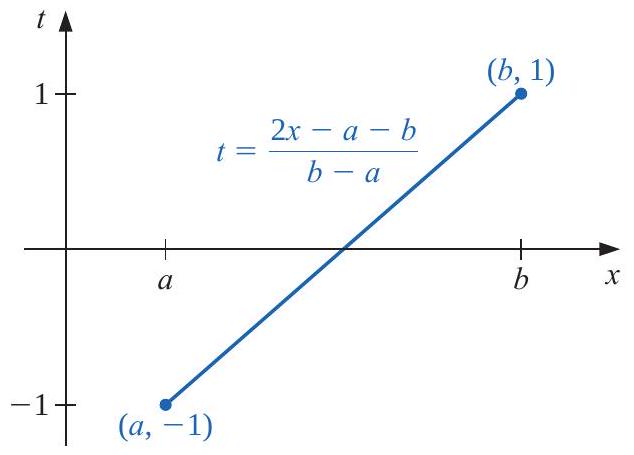
\includegraphics[width=7cm]{2025_05_15_85b7f7df47271a498e1dg-61}
\caption{\scriptsize Figure $6$}
\label{fig:2025_05_15_85b7f7df47271a498e1dg-61}
\end{figure}

This permits Gaussian quadrature to be applied to any interval $[a, b]$, because


\begin{equation}\label{eqn:Gausquad2}
\int_{a}^{b} f(x) d x=\int_{-1}^{1} f\left(\frac{(b-a) t+(b+a)}{2}\right) \frac{(b-a)}{2} d t
\end{equation}


\begin{example}
Consider the integral $\int_{1}^{3} x^{6}-x^{2} \sin (2 x) d x=317.3442466$.\\
\begin{enumerate}[label=(\alph*)]
\item Compare the results for the closed Newton-Cotes formula with $n=1$, the open Newton-Cotes formula with $n=1$, and Gaussian Quadrature when $n=2$.\\
\item Compare the results for the closed Newton-Cotes formula with $n=2$, the open Newton-Cotes formula with $n=2$, and Gaussian Quadrature when $n=3$.
\end{enumerate}
\end{example}

\begin{mysolution}
\begin{enumerate}[label=(\alph*)]
\item Each of the formulas in this part requires 2 evaluations of the function $f(x)=$ $x^{6}-x^{2} \sin (2 x)$. The Newton-Cotes approximations are

$$
\begin{aligned}
\text { Closed } n=1: & \frac{2}{2}[f(1)+f(3)]=731.6054420 \\
\text { Open } n=1: & \frac{3(2 / 3)}{2}[f(5 / 3)+f(7 / 3)]=188.7856682
\end{aligned}
$$

Gaussian quadrature applied to this problem requires that the integral first be transformed into a problem whose interval of integration is $[-1,1]$. Using Eq.\ref{eqn:Gausquad2} gives

$$
\int_{1}^{3} x^{6}-x^{2} \sin (2 x) d x=\int_{-1}^{1}(t+2)^{6}-(t+2)^{2} \sin (2(t+2)) d t
$$

Gaussian quadrature with $n=2$ then gives\\
$\int_{1}^{3} x^{6}-x^{2} \sin (2 x) d x \approx f(-0.5773502692+2)+f(0.5773502692+2)=306.8199344 ;$\\
\item Each of the formulas in this part requires 3 function evaluations. The Newton-Cotes approximations are

$$
\begin{aligned}
\text { Closed } n=2: & \frac{(1)}{3}[f(1)+4 f(2)+f(3)]=333.2380940 \\
\text { Open } n=2: & \frac{4(1 / 2)}{3}[2 f(1.5)-f(2)+2 f(2.5)]=303.5912023
\end{aligned}
$$

Gaussian quadrature with $n=3$, once the transformation has been done, gives

$$
\begin{aligned}
\int_{1}^{3} x^{6}-x^{2} \sin (2 x) d x \approx & 0 . \overline{5} f(-0.7745966692+2)+0 . \overline{8} f(2) \\
& +0 . \overline{5} f(0.7745966692+2)=317.2641516
\end{aligned}
$$

The Gaussian quadrature results are clearly superior in each instance.
\end{enumerate}
\end{mysolution}
%
%Maple has Composite Gaussian Quadrature in the NumericalAnalysis subpackage of Maple's Student package. The default for the number of partitions in the command is 10, so the results in Example 2 would be found for $n=2$ with\\
%$f:=x^{6}-x^{2} \sin (2 x) ; a:=1 ; b:=3:$\\
%Quadrature $(f(x), x=a . . b$, method $=$ gaussian $[2]$, partition $=1$, output $=$ information $)$\\
%which returns the approximation, what Maple assumes is the exact value of the integral, the absolute, and relative errors in the approximations, and the number of function evaluations.
%
%The result when $n=3$ is, of course, obtained by replacing the statement method $=$ gaussian[2] with method = gaussian [3].
\begin{myexercise}%\label{Comprehensionquiz2}
Approximate the following integrals using Gaussian quadrature with $n=2$, and compare your results to the exact values of the integrals.
\begin{multicols}{2}
\begin{enumerate}[label=(\alph*)]
\item $\int_{1}^{1.5} x^{2} \ln x d x$
\item $\int_{0}^{1} x^{2} e^{-x} d x$
\item $\int_{0}^{0.35} \frac{2}{x^{2}-4} d x$
\item $\int_{0}^{\pi / 4} x^{2} \sin x d x$
%\item $\int_{0}^{\pi / 4} e^{3 x} \sin 2 x d x$
%\item $\int_{1}^{1.6} \frac{2 x}{x^{2}-4} d x$
%\item $\int_{3}^{3.5} \frac{x}{\sqrt{x^{2}-4}} d x$
%\item $\int_{0}^{\pi / 4}(\cos x)^{2} d x$
\end{enumerate}
\end{multicols}

\begin{mysolution}
Gaussianquadraturegives:
\begin{multicols}{2}
\begin{enumerate}[label=(\alph*)]
\item $0.1922687$ \item $0.1594104$ \item $-0.1768190$ \item $0.08926302$ 
%\item $2.5913247$ \item $-0.7307230$ \item $0.6361966$ \item $0.6423172$
\end{enumerate}
\end{multicols}
\end{mysolution}
\end{myexercise}


%\discussion


\begin{posttest}[\textcolor{red}{End of Module 5 Quiz}]
\item Approximate $\int_{0}^{2} x^{2} \ln \left(x^{2}+1\right) d x$ using $h=0.25$. Use
\begin{enumerate}[label=(\alph*)]
\item Composite Trapezoidal rule.
\item Composite Simpson's rule.
\item Composite Midpoint rule.
\end{enumerate}

\item Use Romberg integration to compute $R_{4,4}$ for the following integrals.
\begin{multicols}{2}
\begin{enumerate}[label=(\alph*)]
\item  $\quad \int_{1}^{1.5} x^{2} \ln x d x$\\
\item $\int_{0}^{1} x^{2} e^{-x} d x$\\
\item $\quad \int_{0}^{0.35} \frac{2}{x^{2}-4} d x$\\
\item $\quad \int_{0}^{\pi / 4} x^{2} \sin x d x$\\
%\item $\quad \int_{0}^{\pi / 4} e^{3 x} \sin 2 x d x$\\
%\item $\quad \int_{1}^{1.6} \frac{2 x}{x^{2}-4} d x$\\
%\item $\quad \int_{3}^{3.5} \frac{x}{\sqrt{x^{2}-4}} d x$\\
%\item $\int_{0}^{\pi / 4}(\cos x)^{2} d x$
\end{enumerate}
\end{multicols}

\item Use Adaptive quadrature to approximate the following integrals to within $10^{-5}$.
\begin{multicols}{2}
\begin{enumerate}[label=(\alph*)]
\item $\int_{1}^{3} e^{2 x} \sin 3 x d x$\\
\item $\int_{1}^{3} e^{3 x} \sin 2 x d x$\\
\item $\quad \int_{0}^{5}\left(2 x \cos (2 x)-(x-2)^{2}\right) d x$\\
\item $\quad \int_{0}^{5}\left(4 x \cos (2 x)-(x-2)^{2}\right) d x$
\end{enumerate}
\end{multicols}

\item Determine constants $a, b, c$, and $d$ that will produce a quadrature formula

$$
\int_{-1}^{1} f(x) d x=a f(-1)+b f(1)+c f^{\prime}(-1)+d f^{\prime}(1)
$$

that has degree of precision $3$.
\begin{mysolution}
\begin{enumerate}[label=\arabic*.]
\item
\begin{multicols}{3}
\begin{enumerate}[label=(\alph*)]
\item $3.15947567$
\item $3.10933713$
\item $3.00906003$
\end{enumerate}
\end{multicols}

\item
\begin{multicols}{2}
\begin{enumerate}[label=(\alph*)]
\item $0.1922594$ \item $0.1606028$ \item$-0.1768200$ \item $0.08875528$ 
%\item $2.5886272$ \item $-0.7339728$ \item $0.6362134$ \item $0.6426991$
\end{enumerate}
\end{multicols}

\item Adaptive quadrature gives:
\begin{multicols}{2}
\begin{enumerate}[label=(\alph*)]
\item $108.555281$ \item $-1724.966983$  \item$-15.306308$ \item $-18.945949$
\end{enumerate}
\end{multicols}

\item $a =1$, $b =1$, $c = \frac13$, $d =-\frac13$
\end{enumerate}


\end{mysolution}
\end{posttest}

%share your understanding of properties of functions and their applications to solving rates of change problems in physical phenomenon 


%\end{actsoln}

\takehome

\comy{You are now at the last part of this module. Your  task is to do a self-reflection on your learning experience.}



\references
\begin{refenumerate}
\item Kong, Q., Siauw, T., Bayen, A., (2020). Python Programming and Numerical Methods. First Edition, Academic Press,  ISBN-13 ‏ : ‎ 978-0128195499 \\
%chapter 1 pg 7-36 functions\\
%chapter 1 pg 51-83 limits and continuity\\
%chapter 1 pg 45-50 rates of change\\
%chapter 2 pg 108-120 the derivative\\
%\item Mendelson, E. (2022). Schaum's Outline of Calculus. McGraw-Hill Education.
%chapter 6 51-55 functions
%chapter 7 59-65 limits
%chapter 8 69-74 continuity
%chapter 9 77-81 derivative
%\item Calculus \mylink{https://math.libretexts.org/Bookshelves/Calculus}
%\item Chris McMullen, 2021, Essential Calculus Skills Practice Workbook with Full Solutions, Zishka Publishing, ISBN 978-1-941691-24-3
%\item R. Adams and C. Essex, 2021, Calculus: A complete Course, Addison Wesley, ISBN 13: 978-0135732588
%\item P. Abbott and H. Neill, 2018, Calculus: A Complete Introduction: The Easy Way to Learn Calculus (Teach Yourself), ISBN 13: 978-1473678446
\end{refenumerate}





%\wrapup
%To wrap-up, answer the following questions:
%
%\begin{enumerate}
%\item 
%%when do we say that a limit of a function exists?
%%\item how do we remove discontinuity in functions?
%%\item what is the relationship between the gradient of the tangent line and the derivative?
%\end{enumerate}
















%\newpage

%\facilitation


%
\begin{center}
    {\Large \textbf{FUNCTIONS OF SEVERAL VARIABLES}}\\[2mm]
(DEFINITION, DOMAIN, RANGE, GRAPHS AND LEVEL CURVES) \\[4mm]

\mycenterbox{5 minute review}%\\[4mm]
Recap the definition of a function of several variables, and the meaning of domain, range, graph and level curves of functions of several variables.
\end{center}
\mycenterbox{Warm-up.}%\\[4mm]
\problemAnswer{
Match the function with its graph (labeled I–VI).Give reasons for your choices
\begin{multicols}{3}
\begin{enumerate}[label=(\alph*)]
\item $f(x,y)=|x|+|y|$\\[4mm]
\item $f(x,y)=|xy|$
\item $f(x,y)=\frac{1}{1+x^2+y^2}$\\2mm]
\item $f(x,y)=(x^2-y^2)^2$
\item $f(x,y)=(x-y)^2$\\[4mm]
\item $f(x,y)=\sin(|x|+|y|)$
\end{enumerate}
\end{multicols}

\begin{center}
%\centering
\includegraphics[width=10cm]{MCTutorial1Q1.JPEG}
\end{center}
%\tcbox[tcbox raise base]{Warm-up}
 
%\begin{flushright}
%\begin{tikzpicture}
%    % A body
%
%
%    % Non-rectangle shapes must be drawn as polygone
%    \begin{scope}[shift={(3,0)}]
%        \draw  (0,0.5) -- (0,4) -- (.5,4) -- (.5,4.5) -- (1.,4.5) -- (4.,4.5) --(4.,4)-- (4.5,4) --(4.5,0.5) --(4.0,0.5)--(4.0,0.0)-- (.5,0) --(0.5,0.5) -- cycle;
%        % Draw symmetry lines
%        \draw [symmetry] (.5, 0.5) -- (.5,4.0);
%        \draw [symmetry] (4, 0.5) -- (4,4.0);
%        \draw [symmetry] (.5,4.0) -- (4,4.0);
%         \draw [symmetry] (.5, 0.5) -- (4, 0.5);
%        % Dimensions
%        \draw (4.5,0) -- ++(0.5,0) coordinate (D1) -- +(5pt,0);
%        \draw (4.5,4.5) -- ++(0.5,0) coordinate (D2) -- +(5pt,0);
%        \draw [dimen] (D1) -- (D2) node {6cm};
%       
%        
%        \draw (0.0,5) -- ++(0,0.5) coordinate (D1) -- +(0,+5pt);
%        \draw (0.5,5) -- ++(0,0.5) coordinate (D2) -- +(0,+5pt);
%        \draw [dimen,-] (D1) -- (D2) node [above=5pt] {$x$ cm};
%        \draw [dimen,<-] (D1) -- ++(-5pt,0);
%        \draw [dimen,<-] (D2) -- ++(+5pt,0);
%    \end{scope}
%\end{tikzpicture}
%\end{flushright}

}


\mycenterbox{Problems.}%

%\begin{center}
%\tcbox[tcbox raise base]{ Problems. Choose from the below}
%\end{center}
\problem{Exploring functions}%
\begin{enumerate}[(a)]
\item Are the following functions even, odd, or neither? What can you say
about their range?
\begin{multicols}{4}
 \begin{enumerate}[(i)]
\item $\displaystyle \frac{3x}{x^2+2}$
\item $\displaystyle \cos x+3$
\item $\displaystyle \frac{2x^3}{\cos x+3}$
\item $\displaystyle \frac{3x^4+2x^2}{\sin x+4}$
\end{enumerate}
\end{multicols}
\item Consider the functions $\sin^n x$ and $\cos^n x$, where $n$ is a positive integer.
Which are odd, which are even, and what are their periodicities?
\item What is the periodicity of $f(x) = 2 \cos x+\sin 2x$? Is it even/odd/neither?

\end{enumerate}

\problem{Cubic functions} 
Show that $x-1$ is a factor of the cubic function%
$$P(x)=x^3-2x^2-5x+6,$$
and  find the quadratic factor $Q(x)$ such that $P(x) = (x -1)Q(x)$. Factorise
$Q(x)$ and hence sketch $P(x).$

%\newpage
\problem{Sigmoid functions*.}%
For positive integers $n$, consider the family of functions
$$\displaystyle f_n= \frac{x^n}{2^n+x^n}.$$
\begin{enumerate}[(a)]
\item What are appropriate domains and ranges for $f_n(x)$? Do they depend on $n$?

\item Is $f_n(x)$ even, odd, or neither? Does this depend on $n$?

\item Show that for $x\geq 0$, $f_n(x)$ are strictly increasing functions and that
$0\leq f_n(x) < 1.$
\item What is the value of $f_n(2)$? Does it depend on $n$?

\item By considering the values of $f_n(1.9)$ and $f_n(2.1)$ for $n = 2, 4, 8, 16, 32$ and
$64$, show that the graph of $f_n(x)$ for $x\ge 0$ is an increasing sigmoid (that
is, $S$-shaped) function that approaches a step function as $n\rightarrow \infty$.
\end{enumerate}

\mycenterbox{Selected answers and hints}%

For the warm-up, $V(x)=4x(3-x)^2$. Writing $x=1+\epsilon$, we get
$$V = 4(1 +\epsilon)(3- (1+\epsilon))^2=4(4-\epsilon^2(3-\epsilon)).$$
If $-1<\epsilon<2$ then $\epsilon^2 (3-\epsilon)\ge 0$, with equality when $\epsilon=0$. Thus the maximum
value of $V$ occurs when $\epsilon= 0$, i.e. $x = 1\rm{cm}$.

\begin{enumerate}
\item 
\begin{enumerate}[(i)]
\item Odd. The range is the interval  $[-\frac{3}{4}\sqrt{2},\; \frac{3}{4}\sqrt{2}]$
\item Even. The range is the interval $[2, 4]$.
\item Odd. The range is all of $\mathbb R$.
\item Neither. (For example, writing $\displaystyle \frac{5}{\sin x+4}$ we have $\displaystyle f(1)= \frac{5}{\sin (1)+4} \equiv 1.032 (3\rm{dp})$ which is neither $f(1)$ nor $-f(1)$.)\\[4mm]
The range is the nonnegative reals $[0,\infty)$

\end{enumerate}
\end{enumerate}










